
\documentclass[fleqn,addpoints]{exam}
\usepackage{amsmath}
\usepackage{graphicx}
\usepackage{float}
\usepackage{caption}
\usepackage{polynom}
\usepackage{mdwlist}

\everymath{\displaystyle}

\printanswers

\ifprintanswers
\usepackage{2in1, lscape}
\fi

\title{Math 263B Chapter Five Exam}
\date{August 30, 2011}

\begin{document}

\maketitle  

\ifprintanswers
\else
\vspace{0.2in}
\makebox[\textwidth]{Name:\enspace\hrulefill}
\vspace{0.2in}

\begin{center}
\gradetable[h][pages]
\bonusgradetable[h][pages]
\end{center}

\pagebreak

\fi

\begin{questions}

\uplevel{\section{Sums}}
\question[5]
\[
  \sum_{i = 1}^{15} 3i
\]

\begin{solution}[4 cm]
\begin{align*}
  \sum_{i = 1}^{15} 3i &= 3 \sum_{i = 1}^{15} i \\
  &= 3 \cdot \frac{15 \cdot 16}{2} \\
  &= 360 \\
\end{align*}

\end{solution}

\question[7]
\[
\sum_{i = 1}^{10} \left( (i+1)^2 - i^2 \right)
\]

\begin{solution}[4 cm]
Approach 1:
\begin{align*}
  \sum_{i = 1}^{10} \left( (i+1)^2 - i^2 \right) &= (10 + 1)^2 - 1^2 \\
  &= 120 \\
\end{align*}

Approach 2:
\begin{align*}
  \sum_{i = 1}^{10} \left( (i+1)^2 - i^2 \right) &= \sum_{i = 1}^{10} \left( i^2 + 2i + 1 - i^2 \right) \\
  &= \sum_{i = 1}^{10} \left( 2i + 1 \right) \\
  &= 2 \sum_{i = 1}^{10} i +  \sum_{i = 1}^{10} 1 \\
  &= \frac{2 \cdot 10 \cdot 11}{2} + 10 \\
  &= 120 \\
\end{align*}

Approach 3:
\begin{align*}
  \sum_{i = 1}^{10} \left( (i+1)^2 - i^2 \right) &= \sum_{i = 1}^{10} (i + 1)^2 - \sum_{i = 1}^{10} i^2 \\
  &= \sum_{i = 2}^{11} i^2 - \sum_{i = 1}^{10} i^2 \\
  &= \sum_{i = 1}^{10} i^2 + 11^2 - 1^2 - \sum_{i = 1}^{10} i^2 \\
  &= 11^2 - 1^2 \\
  &= 120 \\
\end{align*}

\end{solution}

\uplevel{\section{Indefinite Integrals}}
 
% \uplevel{For questions \ref{indefinite:first} to \ref{indefinite:last}, evaluate the indefinite integrals.}

\question[5]
\label{indefinite:first}
\[
  \int \left( 3x^2 + 5x - \pi^2 \right) \, \mathrm{d}x
\]
\begin{solution}[4 cm]
\[
  \int \left( 3x^2 + 5x - \pi^2 \right) \, \mathrm{d}x = x^3 + \frac{5}{2} x^2 - \pi^2 x + C
\]
\end{solution}

\question[7]
\[
  \int \sin 2x \, \mathrm{d}x
\]

\begin{solution}[5 cm]
\begin{align*}
  u &= 2x \\
  du &= 2 dx \\
\\
  \int \sin 2x \, \mathrm{d}x &= \frac{1}{2} \int \sin u \, \mathrm{d}u \\
  &= -\frac{1}{2} \cos u + C \\
  &= -\frac{1}{2} \cos 2x + C \\
\end{align*}

\end{solution}

\ifprintanswers
\pagebreak
\fi

\question[7]
\[
  \int \frac{4x^3 + 1}{x^2} \, \mathrm{d}x
\]

\begin{solution}[5 cm]
\begin{align*}
  \int \frac{4x^3 + 1}{x^2} \, \mathrm{d}x &= \int \left( 4x + x^{-2} \right) \, \mathrm{d}x \\
  &= 2x^2 - x^{-1} + C \\
  &= 2x^2 - \frac{1}{x} + C \\
\end{align*}

\end{solution}

\question[7]
\[
  \int (x^2 + 2) \sqrt{x^3 + 6x + 2} \, \mathrm{d}x
\]

\begin{solution}[6 cm]

\begin{align*}
  u &= x^3 + 6x + 2 \\
  du &= 3(x^2 + 2) dx \\
\\
  \int (x^2 + 2) \sqrt{x^3 + 6x + 2} \, \mathrm{d}x &= \frac{1}{3} \int u^{1/2} \, \mathrm{d}u \\
  &= \frac{2}{9} u^{3/2} + C \\
  &= \frac{2}{9} (x^3 + 6x + 2)^{3/2} + C \\
\end{align*}

\end{solution}

\ifprintanswers
\pagebreak
\fi

\question[10]
\label{indefinite:last}
\[
  \int \sin^3(x^2 + 1) \cos(x^2 + 1) x  \, \mathrm{d}x
\]

\begin{solution}[7 cm]
\begin{align*}
  u &= \sin(x^2 + 1) \\
  du &= \cos(x^1 + 1) 2x \, dx \\
\\
  \int \sin^3(x^2 + 1) & \cos(x^2 + 1) x \, \mathrm{d}x = \frac{1}{2} \int u^3 \, \mathrm{d}u \\
  &= \frac{1}{8} u^4 \\
  &= \frac{1}{8} \sin^4(x^2 + 1) + C \\
\end{align*}

\end{solution}


\uplevel{\section{Definite Integrals}}
 
% \uplevel{For questions \ref{indefinite:first} to \ref{indefinite:last}, evaluate the indefinite integrals.}

\question[7]
\[
  \int_1^2 \left( 3x^2 - 4x + 3 \right)\, \mathrm{d}x
\]

\begin{solution}[8 cm]
\begin{align*}
  \int_1^2 \left( 3x^2 - 4x + 3 \right)\, \mathrm{d}x &= x^3 - 2x^2 + 3x \bigg|_1^2 \\
  &= 4 \\
\end{align*}
\end{solution}

\pagebreak

\question[7]
\[
  \int_{\pi}^0 (\sin x + \cos x) \, \mathrm{d}x  
\]

\begin{solution}[8 cm]
\begin{align*}
  \int_{\pi}^0 (\sin x + \cos x) \, \mathrm{d}x &= -\cos x + \sin x \bigg|_{\pi}^0 \\
  &= -\cos 0 + \sin 0 - (-\cos \pi + \sin \pi) \\
  &= -2 \\
\end{align*}
\end{solution}

\question[8]
\[
  \int_{1}^{3/2} \cos \pi x  \, \mathrm{d}x
\]

\begin{solution}[8 cm]
\begin{align*}
  u &= \pi x \\
  du &= \pi dx \\
  u(1) &= \pi \\
  u(3/2) &= \frac{3\pi}{2} \\ \\
\\
  \int_1^{3/2} \cos \pi x  \, \mathrm{d}x &= \frac{1}{\pi} \int_{\pi}^{3\pi/2} \cos u \, \mathrm{d}u \\
  &= \frac{1}{\pi} \sin u \bigg|_{\pi}^{3 \pi/2} \\
  &= -\frac{1}{\pi} \\
\end{align*}

\end{solution}

\pagebreak

\question[5]
\[
  \int_{-\pi}^{\pi} x^3 \cos x \, \mathrm{d}x  
\]

\begin{solution}[8 cm]
\[
  f(-x) = (-x)^3 \cos (-x) = -x^3 \cos x = -f(x)
\]

Since this is an odd function, the integral is 0.

\end{solution}

\question[5]
\[
  D_x \left[ \int_1^x \frac{t^2}{\sqrt{3t - 7}} \, \mathrm{d}t \right]
\]
\begin{solution}[8 cm]
\[
  D_x \left[ \int_1^x \frac{t^2}{\sqrt{3t - 7}} \, \mathrm{d}t \right] = \frac{x^2}{\sqrt{3x - 7}} 
\]
\end{solution}

\pagebreak


\question[10]
\[
  D_x \left[ \int_{0}^{\sqrt{x}} t^2 \, \mathrm{d}t \right]
\]
\begin{solution}[8 cm]

approach 1:
\begin{align*}
  u &= x^{1/2} \\
  \frac{du}{dx} &= \frac{1}{2} x^{-1/2} \\
\\
  D_x \left[ \int_{0}^{\sqrt{x}} t^2 \, \mathrm{d}t \right] &= D_u \left[ \int_0^u t^2 \, \mathrm{d}u \right] \cdot \frac{du}{dx} \\
  &= u^2 \cdot \frac{1}{2} x^{-1/2} \\
  &= x \cdot \frac{1}{2} x^{-1/2} \\
  &= \frac{\sqrt{x}}{2} \\
\end{align*}

approach 2:
\begin{align*}
  D_x \left[ \int_{0}^{\sqrt{x}} t^2 \, \mathrm{d}t \right] &= D_x \left[ \frac{t^3}{3} \right|_{0}^{\sqrt{x}} \\
  &= D_x \left[ \frac{x^{3/2}}{3} - 0 \right] \\
  &= \frac{\sqrt{x}}{2} \\
\end{align*}

\end{solution}

\ifprintanswers
\pagebreak
\fi

\question[10]
Find the average value of $f(x) = \frac{x}{(x^2 + 1)^3}$ in the interval $[0, 2]$.

\begin{solution}[5 cm]
First evaluate the integral in the region:
\begin{align*}
  u &= x^2 + 1 \\
  du &= 2x \, dx \\
  u(0) &= 1 \\
  u(2) &= 5 \\
\\
  \int_0^2 \frac{x}{(x^2 + 1)^3} \, \mathrm{d}x &= \frac{1}{2} \int_1^5 u^{-3} \, \mathrm{d}u \\
  &= - \frac{1}{4} u^{-2} \bigg|_1^5 \\
  &= - \frac{1}{4u^2} \bigg|_1^5 \\
  &= - \frac{1}{100} + \frac{1}{4} \\
  &= \frac{6}{25}\\
\end{align*}

The average is the integral divided by the size of the region:
\[
  \frac{1}{2} \cdot \frac{6}{25} = \frac{3}{25}
\]

\end{solution}

\ifprintanswers
\else
\pagebreak
\fi

\uplevel{\section{Extra Credit}}

\bonusquestion[10]

Find the area in the region between the y axis, $y = 2$ and $y = \sqrt{x}$.

\ifprintanswers
\pagebreak
\fi

\begin{solution}[10 cm]

\begin{figure}[H]
  \centering
  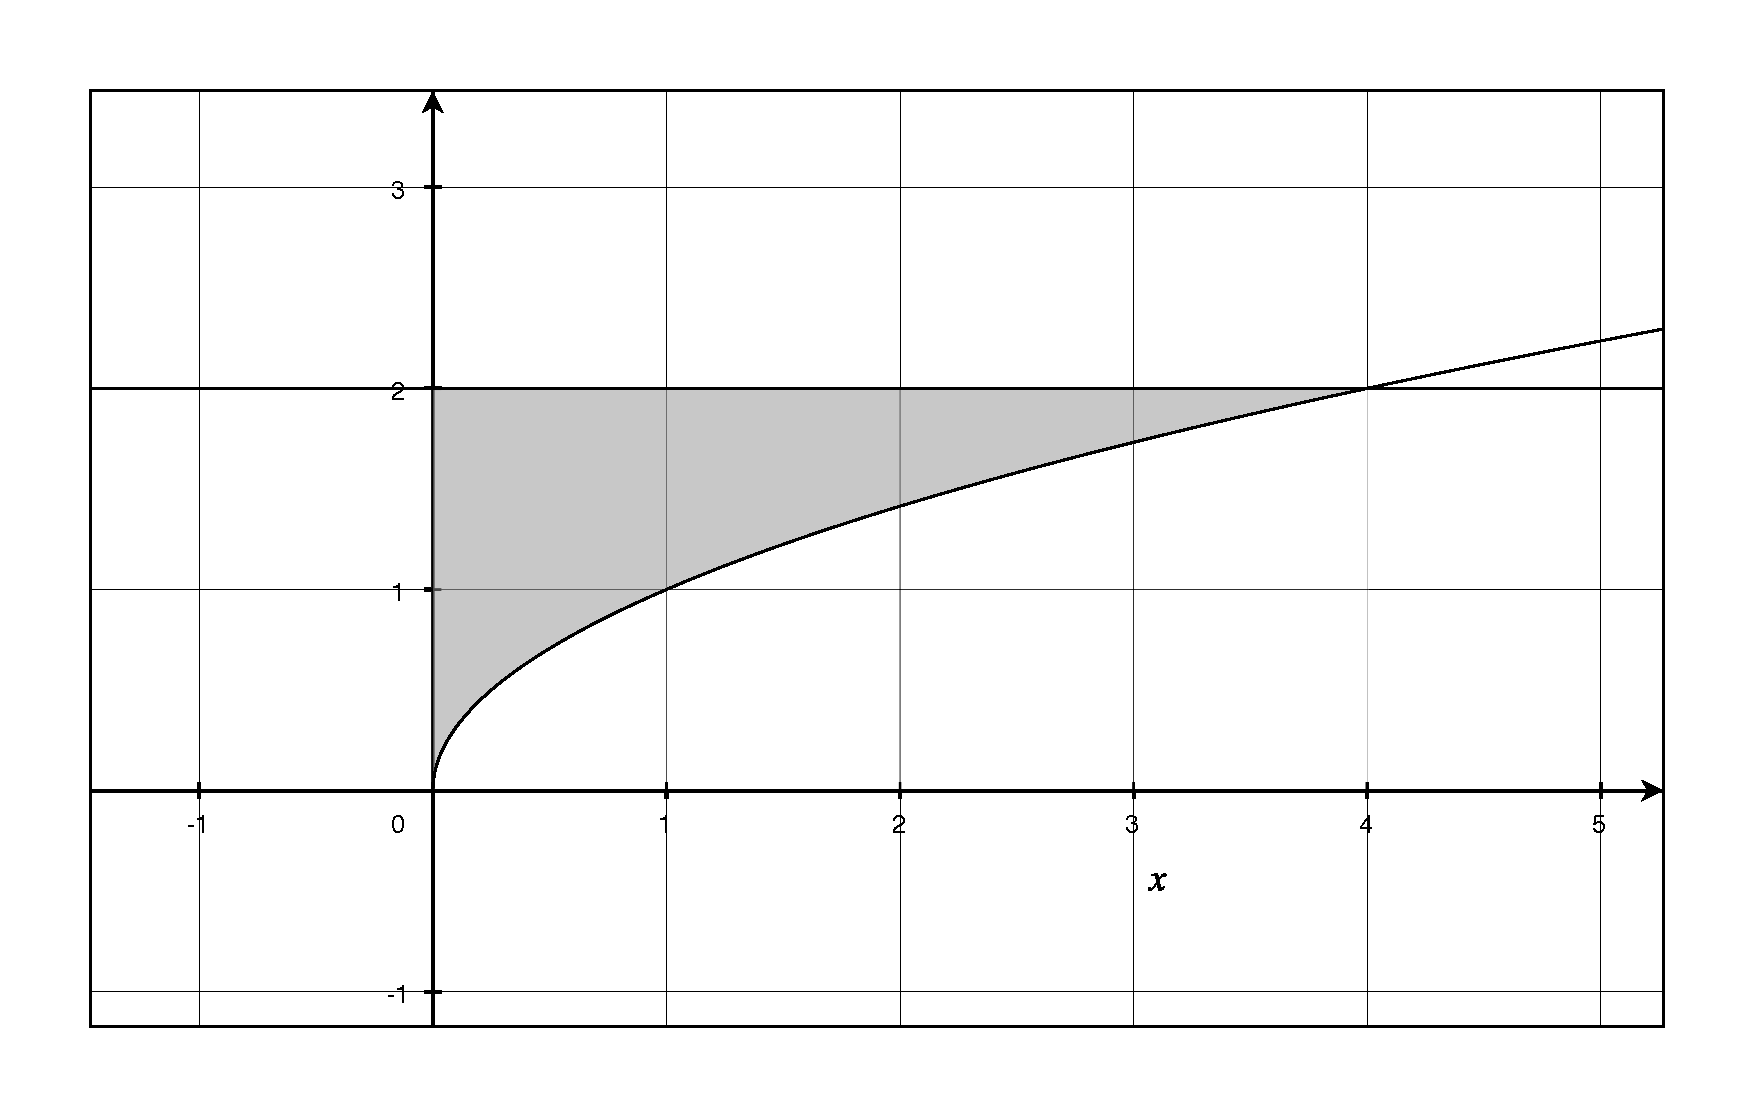
\includegraphics[scale=.3]{extra_credit.eps}
  \caption*{Extra Credit}
\end{figure}

First find the point where the two lines intersect:
\begin{align*}
  \sqrt{x} &= 2 \\
  x &= 4 \\
\end{align*}

The area under $y = \sqrt{x}$ for this region is:
\[
  \int_0^4 x^{1/2} \, \mathrm{d}x = \frac{16}{3}
\]

The area under $y = 2$ is the area of the rectangle or: $4 \cdot 2 = 8$

So the area between the two is the difference:
\[
  A = 8 - \frac{16}{3} = \frac{8}{3}
\]
\end{solution}



\end{questions}

\end{document}
